% Created by tikzDevice version 0.12.6 on 2024-06-15 18:35:03
% !TEX encoding = UTF-8 Unicode
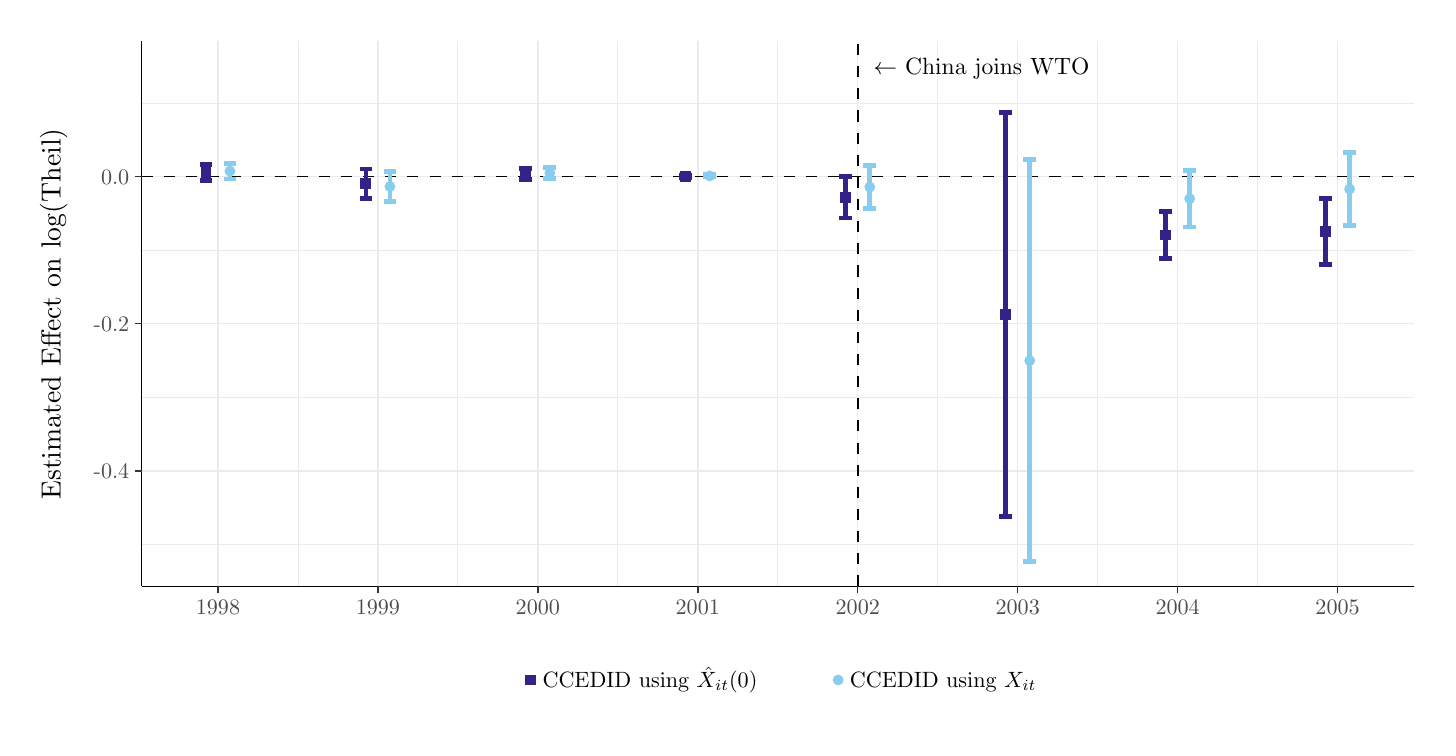
\begin{tikzpicture}[x=1pt,y=1pt]
\definecolor{fillColor}{RGB}{255,255,255}
\path[use as bounding box,fill=fillColor] (0,0) rectangle (505.89,252.94);
\begin{scope}
\path[clip] (  0.00,  0.00) rectangle (505.89,252.94);
\definecolor{drawColor}{RGB}{255,255,255}

\path[draw=drawColor,line width= 0.5pt,line join=round,line cap=round,fill=fillColor] (  0.00, -0.00) rectangle (505.89,252.94);
\end{scope}
\begin{scope}
\path[clip] ( 41.22, 51.02) rectangle (500.89,247.95);
\definecolor{fillColor}{RGB}{255,255,255}

\path[fill=fillColor] ( 41.22, 51.02) rectangle (500.89,247.95);
\definecolor{drawColor}{gray}{0.92}

\path[draw=drawColor,line width= 0.3pt,line join=round] ( 41.22, 66.18) --
	(500.89, 66.18);

\path[draw=drawColor,line width= 0.3pt,line join=round] ( 41.22,119.35) --
	(500.89,119.35);

\path[draw=drawColor,line width= 0.3pt,line join=round] ( 41.22,172.53) --
	(500.89,172.53);

\path[draw=drawColor,line width= 0.3pt,line join=round] ( 41.22,225.70) --
	(500.89,225.70);

\path[draw=drawColor,line width= 0.3pt,line join=round] ( 97.66, 51.02) --
	( 97.66,247.95);

\path[draw=drawColor,line width= 0.3pt,line join=round] (155.46, 51.02) --
	(155.46,247.95);

\path[draw=drawColor,line width= 0.3pt,line join=round] (213.25, 51.02) --
	(213.25,247.95);

\path[draw=drawColor,line width= 0.3pt,line join=round] (271.05, 51.02) --
	(271.05,247.95);

\path[draw=drawColor,line width= 0.3pt,line join=round] (328.85, 51.02) --
	(328.85,247.95);

\path[draw=drawColor,line width= 0.3pt,line join=round] (386.65, 51.02) --
	(386.65,247.95);

\path[draw=drawColor,line width= 0.3pt,line join=round] (444.45, 51.02) --
	(444.45,247.95);

\path[draw=drawColor,line width= 0.5pt,line join=round] ( 41.22, 92.76) --
	(500.89, 92.76);

\path[draw=drawColor,line width= 0.5pt,line join=round] ( 41.22,145.94) --
	(500.89,145.94);

\path[draw=drawColor,line width= 0.5pt,line join=round] ( 41.22,199.11) --
	(500.89,199.11);

\path[draw=drawColor,line width= 0.5pt,line join=round] ( 68.76, 51.02) --
	( 68.76,247.95);

\path[draw=drawColor,line width= 0.5pt,line join=round] (126.56, 51.02) --
	(126.56,247.95);

\path[draw=drawColor,line width= 0.5pt,line join=round] (184.36, 51.02) --
	(184.36,247.95);

\path[draw=drawColor,line width= 0.5pt,line join=round] (242.15, 51.02) --
	(242.15,247.95);

\path[draw=drawColor,line width= 0.5pt,line join=round] (299.95, 51.02) --
	(299.95,247.95);

\path[draw=drawColor,line width= 0.5pt,line join=round] (357.75, 51.02) --
	(357.75,247.95);

\path[draw=drawColor,line width= 0.5pt,line join=round] (415.55, 51.02) --
	(415.55,247.95);

\path[draw=drawColor,line width= 0.5pt,line join=round] (473.35, 51.02) --
	(473.35,247.95);
\definecolor{drawColor}{RGB}{0,0,0}

\path[draw=drawColor,line width= 0.6pt,dash pattern=on 4pt off 4pt ,line join=round] ( 41.22,199.11) -- (500.89,199.11);

\path[draw=drawColor,line width= 0.6pt,dash pattern=on 4pt off 4pt ,line join=round] (299.95, 51.02) -- (299.95,247.95);

\node[text=drawColor,anchor=base west,inner sep=0pt, outer sep=0pt, scale=  0.85] at (305.73,236.05) {$\leftarrow$ China joins WTO};
\definecolor{drawColor}{RGB}{51,34,136}

\path[draw=drawColor,line width= 1.7pt,line join=round] ( 62.11,203.43) --
	( 66.74,203.43);

\path[draw=drawColor,line width= 1.7pt,line join=round] ( 64.42,203.43) --
	( 64.42,197.61);

\path[draw=drawColor,line width= 1.7pt,line join=round] ( 62.11,197.61) --
	( 66.74,197.61);

\path[draw=drawColor,line width= 1.7pt,line join=round] (119.91,201.87) --
	(124.53,201.87);

\path[draw=drawColor,line width= 1.7pt,line join=round] (122.22,201.87) --
	(122.22,191.27);

\path[draw=drawColor,line width= 1.7pt,line join=round] (119.91,191.27) --
	(124.53,191.27);

\path[draw=drawColor,line width= 1.7pt,line join=round] (177.71,202.05) --
	(182.33,202.05);

\path[draw=drawColor,line width= 1.7pt,line join=round] (180.02,202.05) --
	(180.02,198.06);

\path[draw=drawColor,line width= 1.7pt,line join=round] (177.71,198.06) --
	(182.33,198.06);

\path[draw=drawColor,line width= 1.7pt,line join=round] (235.51,199.69) --
	(240.13,199.69);

\path[draw=drawColor,line width= 1.7pt,line join=round] (237.82,199.69) --
	(237.82,198.92);

\path[draw=drawColor,line width= 1.7pt,line join=round] (235.51,198.92) --
	(240.13,198.92);

\path[draw=drawColor,line width= 1.7pt,line join=round] (293.31,199.12) --
	(297.93,199.12);

\path[draw=drawColor,line width= 1.7pt,line join=round] (295.62,199.12) --
	(295.62,184.19);

\path[draw=drawColor,line width= 1.7pt,line join=round] (293.31,184.19) --
	(297.93,184.19);

\path[draw=drawColor,line width= 1.7pt,line join=round] (351.10,222.22) --
	(355.73,222.22);

\path[draw=drawColor,line width= 1.7pt,line join=round] (353.42,222.22) --
	(353.42, 76.39);

\path[draw=drawColor,line width= 1.7pt,line join=round] (351.10, 76.39) --
	(355.73, 76.39);

\path[draw=drawColor,line width= 1.7pt,line join=round] (408.90,186.51) --
	(413.53,186.51);

\path[draw=drawColor,line width= 1.7pt,line join=round] (411.22,186.51) --
	(411.22,169.51);

\path[draw=drawColor,line width= 1.7pt,line join=round] (408.90,169.51) --
	(413.53,169.51);

\path[draw=drawColor,line width= 1.7pt,line join=round] (466.70,191.09) --
	(471.33,191.09);

\path[draw=drawColor,line width= 1.7pt,line join=round] (469.01,191.09) --
	(469.01,167.33);

\path[draw=drawColor,line width= 1.7pt,line join=round] (466.70,167.33) --
	(471.33,167.33);
\definecolor{drawColor}{RGB}{136,204,238}

\path[draw=drawColor,line width= 1.7pt,line join=round] ( 70.78,203.94) --
	( 75.40,203.94);

\path[draw=drawColor,line width= 1.7pt,line join=round] ( 73.09,203.94) --
	( 73.09,198.26);

\path[draw=drawColor,line width= 1.7pt,line join=round] ( 70.78,198.26) --
	( 75.40,198.26);

\path[draw=drawColor,line width= 1.7pt,line join=round] (128.58,200.98) --
	(133.20,200.98);

\path[draw=drawColor,line width= 1.7pt,line join=round] (130.89,200.98) --
	(130.89,190.06);

\path[draw=drawColor,line width= 1.7pt,line join=round] (128.58,190.06) --
	(133.20,190.06);

\path[draw=drawColor,line width= 1.7pt,line join=round] (186.38,202.35) --
	(191.00,202.35);

\path[draw=drawColor,line width= 1.7pt,line join=round] (188.69,202.35) --
	(188.69,198.55);

\path[draw=drawColor,line width= 1.7pt,line join=round] (186.38,198.55) --
	(191.00,198.55);

\path[draw=drawColor,line width= 1.7pt,line join=round] (244.18,199.79) --
	(248.80,199.79);

\path[draw=drawColor,line width= 1.7pt,line join=round] (246.49,199.79) --
	(246.49,198.98);

\path[draw=drawColor,line width= 1.7pt,line join=round] (244.18,198.98) --
	(248.80,198.98);

\path[draw=drawColor,line width= 1.7pt,line join=round] (301.98,203.13) --
	(306.60,203.13);

\path[draw=drawColor,line width= 1.7pt,line join=round] (304.29,203.13) --
	(304.29,187.55);

\path[draw=drawColor,line width= 1.7pt,line join=round] (301.98,187.55) --
	(306.60,187.55);

\path[draw=drawColor,line width= 1.7pt,line join=round] (359.77,205.24) --
	(364.40,205.24);

\path[draw=drawColor,line width= 1.7pt,line join=round] (362.09,205.24) --
	(362.09, 59.97);

\path[draw=drawColor,line width= 1.7pt,line join=round] (359.77, 59.97) --
	(364.40, 59.97);

\path[draw=drawColor,line width= 1.7pt,line join=round] (417.57,201.40) --
	(422.20,201.40);

\path[draw=drawColor,line width= 1.7pt,line join=round] (419.89,201.40) --
	(419.89,180.86);

\path[draw=drawColor,line width= 1.7pt,line join=round] (417.57,180.86) --
	(422.20,180.86);

\path[draw=drawColor,line width= 1.7pt,line join=round] (475.37,207.88) --
	(480.00,207.88);

\path[draw=drawColor,line width= 1.7pt,line join=round] (477.68,207.88) --
	(477.68,181.41);

\path[draw=drawColor,line width= 1.7pt,line join=round] (475.37,181.41) --
	(480.00,181.41);
\definecolor{fillColor}{RGB}{51,34,136}

\path[fill=fillColor] ( 62.46,198.56) --
	( 66.39,198.56) --
	( 66.39,202.48) --
	( 62.46,202.48) --
	cycle;

\path[fill=fillColor] (120.26,194.61) --
	(124.18,194.61) --
	(124.18,198.53) --
	(120.26,198.53) --
	cycle;

\path[fill=fillColor] (178.06,198.10) --
	(181.98,198.10) --
	(181.98,202.02) --
	(178.06,202.02) --
	cycle;

\path[fill=fillColor] (235.86,197.34) --
	(239.78,197.34) --
	(239.78,201.27) --
	(235.86,201.27) --
	cycle;

\path[fill=fillColor] (293.66,189.69) --
	(297.58,189.69) --
	(297.58,193.61) --
	(293.66,193.61) --
	cycle;

\path[fill=fillColor] (351.45,147.34) --
	(355.38,147.34) --
	(355.38,151.27) --
	(351.45,151.27) --
	cycle;

\path[fill=fillColor] (409.25,176.05) --
	(413.18,176.05) --
	(413.18,179.97) --
	(409.25,179.97) --
	cycle;

\path[fill=fillColor] (467.05,177.25) --
	(470.98,177.25) --
	(470.98,181.17) --
	(467.05,181.17) --
	cycle;
\definecolor{fillColor}{RGB}{136,204,238}

\path[fill=fillColor] ( 73.09,201.10) circle (  1.96);

\path[fill=fillColor] (130.89,195.52) circle (  1.96);

\path[fill=fillColor] (188.69,200.45) circle (  1.96);

\path[fill=fillColor] (246.49,199.38) circle (  1.96);

\path[fill=fillColor] (304.29,195.34) circle (  1.96);

\path[fill=fillColor] (362.09,132.61) circle (  1.96);

\path[fill=fillColor] (419.89,191.13) circle (  1.96);

\path[fill=fillColor] (477.68,194.65) circle (  1.96);
\end{scope}
\begin{scope}
\path[clip] (  0.00,  0.00) rectangle (505.89,252.94);
\definecolor{drawColor}{RGB}{0,0,0}

\path[draw=drawColor,line width= 0.5pt,line join=round] ( 41.22, 51.02) --
	( 41.22,247.95);
\end{scope}
\begin{scope}
\path[clip] (  0.00,  0.00) rectangle (505.89,252.94);
\definecolor{drawColor}{gray}{0.30}

\node[text=drawColor,anchor=base east,inner sep=0pt, outer sep=0pt, scale=  0.80] at ( 36.72, 90.01) {-0.4};

\node[text=drawColor,anchor=base east,inner sep=0pt, outer sep=0pt, scale=  0.80] at ( 36.72,143.18) {-0.2};

\node[text=drawColor,anchor=base east,inner sep=0pt, outer sep=0pt, scale=  0.80] at ( 36.72,196.36) {0.0};
\end{scope}
\begin{scope}
\path[clip] (  0.00,  0.00) rectangle (505.89,252.94);
\definecolor{drawColor}{gray}{0.20}

\path[draw=drawColor,line width= 0.5pt,line join=round] ( 38.72, 92.76) --
	( 41.22, 92.76);

\path[draw=drawColor,line width= 0.5pt,line join=round] ( 38.72,145.94) --
	( 41.22,145.94);

\path[draw=drawColor,line width= 0.5pt,line join=round] ( 38.72,199.11) --
	( 41.22,199.11);
\end{scope}
\begin{scope}
\path[clip] (  0.00,  0.00) rectangle (505.89,252.94);
\definecolor{drawColor}{RGB}{0,0,0}

\path[draw=drawColor,line width= 0.5pt,line join=round] ( 41.22, 51.02) --
	(500.89, 51.02);
\end{scope}
\begin{scope}
\path[clip] (  0.00,  0.00) rectangle (505.89,252.94);
\definecolor{drawColor}{gray}{0.20}

\path[draw=drawColor,line width= 0.5pt,line join=round] ( 68.76, 48.52) --
	( 68.76, 51.02);

\path[draw=drawColor,line width= 0.5pt,line join=round] (126.56, 48.52) --
	(126.56, 51.02);

\path[draw=drawColor,line width= 0.5pt,line join=round] (184.36, 48.52) --
	(184.36, 51.02);

\path[draw=drawColor,line width= 0.5pt,line join=round] (242.15, 48.52) --
	(242.15, 51.02);

\path[draw=drawColor,line width= 0.5pt,line join=round] (299.95, 48.52) --
	(299.95, 51.02);

\path[draw=drawColor,line width= 0.5pt,line join=round] (357.75, 48.52) --
	(357.75, 51.02);

\path[draw=drawColor,line width= 0.5pt,line join=round] (415.55, 48.52) --
	(415.55, 51.02);

\path[draw=drawColor,line width= 0.5pt,line join=round] (473.35, 48.52) --
	(473.35, 51.02);
\end{scope}
\begin{scope}
\path[clip] (  0.00,  0.00) rectangle (505.89,252.94);
\definecolor{drawColor}{gray}{0.30}

\node[text=drawColor,anchor=base,inner sep=0pt, outer sep=0pt, scale=  0.80] at ( 68.76, 41.01) {1998};

\node[text=drawColor,anchor=base,inner sep=0pt, outer sep=0pt, scale=  0.80] at (126.56, 41.01) {1999};

\node[text=drawColor,anchor=base,inner sep=0pt, outer sep=0pt, scale=  0.80] at (184.36, 41.01) {2000};

\node[text=drawColor,anchor=base,inner sep=0pt, outer sep=0pt, scale=  0.80] at (242.15, 41.01) {2001};

\node[text=drawColor,anchor=base,inner sep=0pt, outer sep=0pt, scale=  0.80] at (299.95, 41.01) {2002};

\node[text=drawColor,anchor=base,inner sep=0pt, outer sep=0pt, scale=  0.80] at (357.75, 41.01) {2003};

\node[text=drawColor,anchor=base,inner sep=0pt, outer sep=0pt, scale=  0.80] at (415.55, 41.01) {2004};

\node[text=drawColor,anchor=base,inner sep=0pt, outer sep=0pt, scale=  0.80] at (473.35, 41.01) {2005};
\end{scope}
\begin{scope}
\path[clip] (  0.00,  0.00) rectangle (505.89,252.94);
\definecolor{drawColor}{RGB}{0,0,0}

\node[text=drawColor,rotate= 90.00,anchor=base,inner sep=0pt, outer sep=0pt, scale=  1.00] at ( 11.89,149.48) {Estimated Effect on $\log($Theil$)$};
\end{scope}
\begin{scope}
\path[clip] (  0.00,  0.00) rectangle (505.89,252.94);
\definecolor{fillColor}{RGB}{255,255,255}

\path[fill=fillColor] (162.58,  5.00) rectangle (379.52, 29.45);
\end{scope}
\begin{scope}
\path[clip] (  0.00,  0.00) rectangle (505.89,252.94);
\definecolor{fillColor}{RGB}{255,255,255}

\path[fill=fillColor] (167.58, 10.00) rectangle (196.04, 24.45);
\end{scope}
\begin{scope}
\path[clip] (  0.00,  0.00) rectangle (505.89,252.94);
\definecolor{fillColor}{RGB}{51,34,136}

\path[fill=fillColor] (179.85, 15.26) --
	(183.77, 15.26) --
	(183.77, 19.19) --
	(179.85, 19.19) --
	cycle;
\end{scope}
\begin{scope}
\path[clip] (  0.00,  0.00) rectangle (505.89,252.94);
\definecolor{fillColor}{RGB}{255,255,255}

\path[fill=fillColor] (278.66, 10.00) rectangle (307.12, 24.45);
\end{scope}
\begin{scope}
\path[clip] (  0.00,  0.00) rectangle (505.89,252.94);
\definecolor{fillColor}{RGB}{136,204,238}

\path[fill=fillColor] (292.89, 17.23) circle (  1.96);
\end{scope}
\begin{scope}
\path[clip] (  0.00,  0.00) rectangle (505.89,252.94);
\definecolor{drawColor}{RGB}{0,0,0}

\node[text=drawColor,anchor=base west,inner sep=0pt, outer sep=0pt, scale=  0.80] at (186.04, 14.47) {CCEDID using $\hat{X}_{it}(0)$};
\end{scope}
\begin{scope}
\path[clip] (  0.00,  0.00) rectangle (505.89,252.94);
\definecolor{drawColor}{RGB}{0,0,0}

\node[text=drawColor,anchor=base west,inner sep=0pt, outer sep=0pt, scale=  0.80] at (297.12, 14.47) {CCEDID using $X_{it}$};
\end{scope}
\end{tikzpicture}
